
\subsection{Ring-LWE}
One of the recurring problems in lattice-based cryptography is the key-size and general efficiency. In the GGH cryptosystem, the key-size is $\tilde{O}(n^4)$. In the system based on the hardness of LWE presented in the previous section, the size is in the range of $\tilde{O}(n^2)$\footnote{There are $m$ samples of length $n$. Turns out that for $m > n$, the problem can become only easier, but the same holds for $m \ll n$. Therefore, in most applications, $m$ is chosen to be roughly the size of $n$.}. As we will also see later, there is some minimal efficiency needed for the scheme in order to enable the boostrapping (for FHE). Unfortunately, none of the schemes presented so far satisfy those criterions and so, we need to look for something better.

One idea to improve the efficiency, is to assume some underlying structure of the space we are performing computations in. For example, we can assume that the $\bm{a}$ vectors from previous section are given to us in block of $n$ samples $\bm{a}_1, \bm{a}_2, \dots, \bm{a}_n \in \Z_q^n$ where all of the elements are related. Namely, $\bm{a}_1 = (a_1, \dots, a_n)$ is again chosen uniformly but each $\bm{a}_i = (a_i, \dots, a_n, -a_1, \dots, -a_{i - 1})$ is a ``anti-cyclic'' of the initial $\bm{a}_1$. This choice seems rather arbitrary however we will show how it is a natural consequence of everything we did so far and yields arguably the best results. For example if $n = 4$ and $q = 17$ and $\bm{a}_1 = (1, 16, 4, 5)$ as before, then $\bm{a}_3$ has the form $(4, 5, -1, -16) = (4, 5, 16, 1)$. Note that representing $n$ vectors now takes only $O(n)$ elements from $\Z_q$ rather than $O(n^2)$. The underlying structure is a ring, hence the name ring-LWE (or R-LWE), that is, we replace the group $\Z_q^n$ by picking some ring $R$ of degree $n$ over $\Z$ and a positive modulus $q$ defining the quotient ring $R_q := R/qR$. In most of the cases (as well as in this exposition), $R$ is taken to be a \textit{cyclotomic} ring - i.e. $R_q = \Z_q[x]/\langle x^n + 1 \rangle$ for $n = 2^k$ which turns out to yield much simpler proofs for slightly weaker results.

In the year 2010, Vadim Lyubashevski, Chris Peikert and Oded Regev presented their paper ``On Ideal Lattices and Learning With Errors Over Rings'' \cite{ring-lwe}. The main purpose of the paper was to ``translate'' the LWE problem onto a ring as was done with the SIS problem (mainly by Micciancio \cite{ring-sis} that was followed up by other works but these results are not presented in this paper) and followed the heuristic approach behind the NTRU\footnote{As mentioned by Peikert in his survey: ``The meaning of the acronym NTRU is somewhat mysterious; plausible candidates include "$N$th degree \textit{tru}ncated polynomial ring" and "Number Theorists ’R’ Us."'' - \cite{lattice-survey}} cryptosystem \cite{ntru}. This in particular means first, defining the ring-LWE and later proving the hardness based on some difficult lattice problems like \prob{SVP} along with pseudorandomness of the ring-LWE distribution (analogous to \ref{s-to-d} whose definition will appear later). The second issue turned out to be quite nontrivial and required good insight in the algebraic number theory as well as Gaussian measures and distributions.

Somewhat analogous to the previous section, this one is also split into two main parts. First part - Section \ref{h-rlwe} - focuses on the hardness of the search version of the RLWE. The approach is identical to the one presented for the standard LWE. However, one needs to pay attention to details that are implied by the shift to $R$ like for example the shape of the error distribution under the canonical embedding. Fortunately for us, the quantum part of the reduction can be adopted almost as is and so, we will only mention it briefly. The second part - Section \ref{pseudo-rlwe} - deals with pseudorandomness of the RLWE distribution and thus proving the equivalence between the search and decision versions. This one will require much more insight into the algebraic number theory compared to any other part of this paper and so, we will discuss it in much more detail. Before we dwell any further, we need to establish some terminology and useful lemmas. This is done in the following section.

\subsubsection{Background III}
We begin this section by specifying some details on the underlying ring along with the definitions of the RLWE distribution analogous to the section on standard LWE. We could not find one single source that would cover all of the details necessary, however a good choice would be \cite{algebra}, \cite{stein} or \cite{milne}. For a good discussion on the different idal, see Keith Conrads \href{https://kconrad.math.uconn.edu/blurbs/gradnumthy/different.pdf}{paper}.

In this exposition, we will simplify few details of the proofs and definitions by taking harder assumptions on the underlying structures. For example, our underlying number field will be cyclotomic, i.e. a field extension $K=\Q(\zeta_m)$ obtained by adjoining an element $\zeta_m$ of order $m$ (a primitive $m$th root of unity) to the rationals. For such field, its ring of integers happens to be $R := \Oo_K = \Z[\zeta_m] \cong \Z[X]/\Phi_m(X)$ and so, it is generated by the set $\{\zeta_m^j\}_{j \in [n]}$ (also called the power basis). Furthermore, we fix $m = 2^k$ for some $k \geq 1$ and motivate this choice in \ref{why?}.

\paragraph{Algebraic Number Theory II}
\begin{definition}[Trace]
\end{definition}
\begin{definition}[Norm]
\end{definition}
rings of integers
\begin{definition}[The space H]
\end{definition}
\begin{definition}[Canonical embedding]
\end{definition}
\begin{definition}[Dual]
\end{definition}

\pinar{For cyclotomic fields, how does this dual look like?}

\paragraph{Why cyclotomic?}\label{why?}
As mentioned earlier, we wish to fix the degree of our cyclotomic polynomial to a power-of-two. This leads to greatly simplified proofs of some results like for example search-to-decision reduction in section \ref{pseudo-rlwe}. Nonetheless, in places where it is not necessary, we will be using arbitrary number fields, sometimes not even cyclotomic. We will now list few desirable properties of cyclotomic rings (also those of power of two) that will be useful for us later on. Let us fix $m$, $n$ and $k$ to some positive integers.
\begin{itemize}
	\item Under the canonical embedding, the cyclotomic ring $R = \Oo_K$ for $\Phi_m(x) = x^{\phi(m)} - 1$ embeds as a lattice which in general, is not self-dual (this is only the case for $\Z^n$). Instead, its dual lattice corresponds to a fractional ideal $\Rd \subset K$ such that $R \subseteq \Rd \subseteq m^{-1}R$. In the case where $n = \varphi(m) =  2^{k-1}$ these two are actually equivalent, namely $\Rd = n^{-1}R$. 
	\item Polynomial arithmetic modulo $\Phi_m(X)$ can be performed very efficiently using slightly adjusted, classical $n$-dimensional FFT - \cite{toolkit}, \cite{swift}.
	\item In general, the smaller the shortest vector $\lambda_1(\Ll)$ is, the less secure the system. Cyclotomic fields have relatively large $\lambda_1(\Rd)$ - \cite{oracle}.
	\item In fact, for $n = 2^k$, we have $\lambda_n(\Rd) = 1/\sqrt{n}$
		\iffalse
	\item They also have relatively small \textit{expansion factors} (roughly speaking it is the ratio of the size of the public key to the size of the secret key) as defined and explained in \cite{expansion}.
		\fi
\end{itemize}
Unfortunately, cyclotomic fields with degree of a power-of-two are quite rare and restrictive. Imagine that our system is deemed insecure for some large $n = 2^k$. It might so happen that the next power of two is completely impractical when implemented. We should be able to find something inbetween the two instead.
Cyclotomic number fields have \textit{Galois} group
\paragraph{The RLWE distribution}

\pinar{Add explicit examples?? Fix a quadratic field $\Q(\zeta_3)$ or $\Q(\sqrt{-1})$ and so on.}

\begin{definition}[Ring-LWE Distribution]
	For $s \in \Rd_q$ (the ``secret'') and an error distribution $\psi$ over $K_{\R}$, a sample from the ring-LWE distribution $A_{s, \psi}$ over $R_q \cross \T$ is generated by choosing $a \leftarrow R_q$ uniformly at random, choosing $e \leftarrow \psi$, and outputting $(a, b = (a \cdot s)/q + e \mod \Rd)$.
\end{definition}
\begin{definition}[Ring-LWE, Search)]
	Let $\Psi$ be a family of distributions over $K_{\R}$. The search version of the ring-LWE problem, denoted R-LWE$_{q, \Psi}$, is defined as follows: given access to arbitrarily many independent samples from $A_{s, \psi}$ for some arbitrary $s \in \Rd_q$ and $\psi \in \Psi$, find $s$.
\end{definition}
\subsubsection{Hardness of search Ring-LWE}\label{h-rlwe}
We can finally discuss the main results from the \cite{ring-lwe}. This section focuses on the quantum reduction from $R$-LWE$_{q, \Psi_{\leq \alpha}}$ to the $K$-DGS$_{\gamma}$ - the approximate (to within $\gamma$) discrete Gaussian sampling problem (the definition for an arbitrary number field $K$ is created by simply replacing the lattice $\Ll$ with an ideal $\I$ in Definition \ref{dgs}, and so, the samples are defined to be from D$_{\I, r}$.). Note that all the results from this section apply to general number fields, not only cyclotomic.

The following is an equivalent of Theorem \ref{heart} of the classical LWE. Statement is almost identical however the proof turns out to be much more difficult to achieve than it may look at the first glimpse.
\begin{theorem}
	Let $K$ be an arbitrary number field of degree $n$ and $R = \Oo_K$. Let $\alpha = \alpha(n) > 0$, and let $q = q(n) \geq 2$ be such that $\alpha q > 2 \sqrt{n}$. For some negligible $\epsilon = \epsilon(n)$, there is a probabilistic polynomial-time quantum reduction from $K$-DGS$_{\gamma}$ to $R$-LWE$_{q,\Psi_{\leq \alpha}}$ where $\gamma > 0$ is usually taken\footnote{See the discussion just before Section 4.1 in \cite{ring-lwe}.} to be $\gamma = \omega(\log n)$.
\end{theorem}
And just as before, the proof relies on the (adjusted) \textit{iterative step} (IS) in parallel with the previous section. It presents as follows.
\begin{lemma}[Iterative Step]
Let $\epsilon = \epsilon(n)$ be a negligible function, $\alpha > 0$ real, and $q \geq 2$ be an integer. Assume that we have access to an oracle that solves LWE$_{q, \Psi_{\leq \alpha}}$ given a polynomial number of samples. Then, there exists an efficient quantum algorithm that, given a fractional ideal $\I$ in $K$, a number $r > \sqrt{2}q \cdot \eta_{\epsilon}(\I)$ and a (polynomial) list of samples from the discrete Gaussian distribution D$_{\I,r}$, produces a sample from D$_{\I,r \cdot \gamma/(\alpha q)}$.	
\end{lemma}
It is easy to notice that the statement is almost identical to the Lemma \ref{is}. The place of a $n$-dimensional lattice $\Ll$ has been taken up by a fractional ideal $\I$ (which, when embedded, lives in $\C^n$ as an $n$-dimensional lattice). The proof is also almost intact. We will use Lemma \ref{classical-rlwe} and Lemma \ref{quantum-rlwe} to create a sequence of discrete Gaussians with decreasing radii to obtain the solution to $K$-DGS$_{\gamma}$.
\begin{lemma}[Step 1 - classical]\label{classical-rlwe}
	Let $\epsilon = \epsilon(n)$ be a negligible function, $\alpha > 0$ real, and $q \geq 2$ be an integer with known factorization. Let $\I$ be a fractional ideal in $K$, and let $r \geq \sqrt{2}q \cdot \eta_{\epsilon}(\I)$. Given polynomial list of samples from the discrete Gaussian distribution D$_{\I,r}$, there is a probabilistic polynomial-time (classical) reduction from \prob{CVP}$_{\I^{\vee},d}$ to $R$-LWE$_{q,\Psi_{\leq \alpha}}$, where $d = \alpha q/(\sqrt{2}r)$.
\end{lemma}
\begin{remark}
	In the original statement in \cite{ring-lwe}, \prob{CVP} is replaced by \prob{BDD} to within the same distance. These statements are very similar with a simple difference that \prob{BDD} is concerned with finding \textit{any} lattice vector within $d$ whereas \prob{CVP} wants to find the \textit{closest} vector. Since the distance $d$ is less than $\lambda_1(\Ll)/2$, \prob{BDD} will find the closest, unique vector to $\Ll$. Hence, in this case, they are equivalent and we use \prob{CVP} to keep it consistent with previous section.
\end{remark}

We will proof the lemma using three steps.
\begin{proof}
	Just as before, it is enough to show reduction to \prob{CVP}$^{(q)}_{\I,d}$ by a similar argument. The high-lever reduction presents now as follows. We are given a \prob{CVP}$_{\I, d}$ instance $y = x + e$ where $x \in \Id$ and $\norm{e} \leq d$. We are also granted access to (as many as necessary) samples from the discrete Gaussian over $\I$ and standard deviation $r$ as well as an oracle for $R$-LWE \krzys{why do they not require an oracle for LWE in the assumptions?}\krzys{also, why do we need the theta u if the z is already taken from ideal I?}
\end{proof}
\subsubsection{Pseudorandomness of Ring-LWE}\label{pseudo-rlwe}
Just like in the case of classical LWE, we want to show that the ring-LWE distribution is pseudorandom - i.e. samples from the RLWE distribution are indistinguishable from truly random (uniform) ones. This is encapsulated in the following theorem. Thus far, let us fix some terminology. 
\begin{theorem}
	Let $R$ and $q$ be as above and let $\alpha q \geq \eta_{\epsilon}(\Rd)$ for some negligible $\epsilon = \epsilon(n)$. Then there is a reduction from $R$-LWE$_{q,\Psi_{\leq \alpha}}$ to $R$-DLWE$_{q,\D_{\xi}}$
\end{theorem}
The reduction follows from search-$R$-LWE to decision-$R$-LWE and in high-level description consists of following steps.\\
\begin{enumerate}
	\item (1)
\end{enumerate}

\begin{centering}
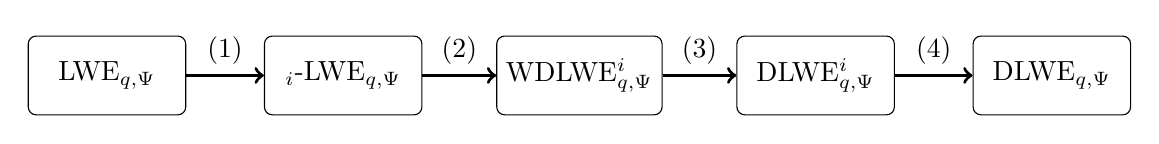
\begin{tikzpicture}
% Define the first acronym
	\node[draw, rounded corners=1mm, minimum width=2cm, minimum height=1cm] (A) at (0,0) {LWE$_{q, \Psi}$};

% Define the second acronym
	\node[draw, rounded corners=1mm, minimum width=2cm, minimum height=1cm] (B) at (3,0) {$\q_i$-LWE$_{q, \Psi}$};

% Define the third acronym
	\node[draw, rounded corners=1mm, minimum width=2cm, minimum height=1cm] (C) at (6,0) {WDLWE$^i_{q, \Psi}$};

% Define the fourth acronym
	\node[draw, rounded corners=1mm, minimum width=2cm, minimum height=1cm] (D) at (9,0) {DLWE$^i_{q, \Psi}$};

% Define the fifth acronym
	\node [draw, rounded corners=1mm, minimum width=2cm, minimum height=1cm] (E) at (12,0) {DLWE$_{q, \Psi}$};

% Draw the arrows between the acronyms
	\draw[->, very thick] (A.east) -- node [above] {(1)} (B.west);
	\draw[->, very thick] (B.east) -- node [above] {(2)} (C.west);
	\draw[->, very thick] (C.east) -- node [above] {(3)} (D.west);
	\draw[->, very thick] (D.east) -- node [above] {(4)} (E.west);
\end{tikzpicture}
\end{centering}


Chinese remainder theorem for rings --> Thm II.4.12 in Top's lecture notes. \\
For instance, they have unique factorization of ideals, and their fractional ideals form a multiplicative group; in general, neither property holds in $\Z[x]/\langle f (x) \rangle$ for monic irreducible $f (x)$, as demonstrated by the ring $\Z[x]/\langle x^2+3 \rangle = \Z[\sqrt{-3}]$. (For example, in this ring $4 = 22 = (1+\sqrt{-3})(1 - \sqrt{-3})$, but 2, $1 + \sqrt{-3}$, and $1 - \sqrt{-3}$ are all irreducible.)
Toward basing fully homomorphic encryption on worst-case hardness \\
One of the applications is \cite{qTESLA} signature scheme.
